% \documentclass[varwidth, border=0.125in]{standalone}
\documentclass[a4paper]{article}
\usepackage[cm]{fullpage}
\usepackage{graphicx}
% \usepackage{subfig}
% \usepackage{subfloat}
\usepackage{subcaption}

\begin{document}
\begin{figure}[!h]
  \centering
  \begin{subfigure}[t]{0.45\linewidth}
    \begin{center}
    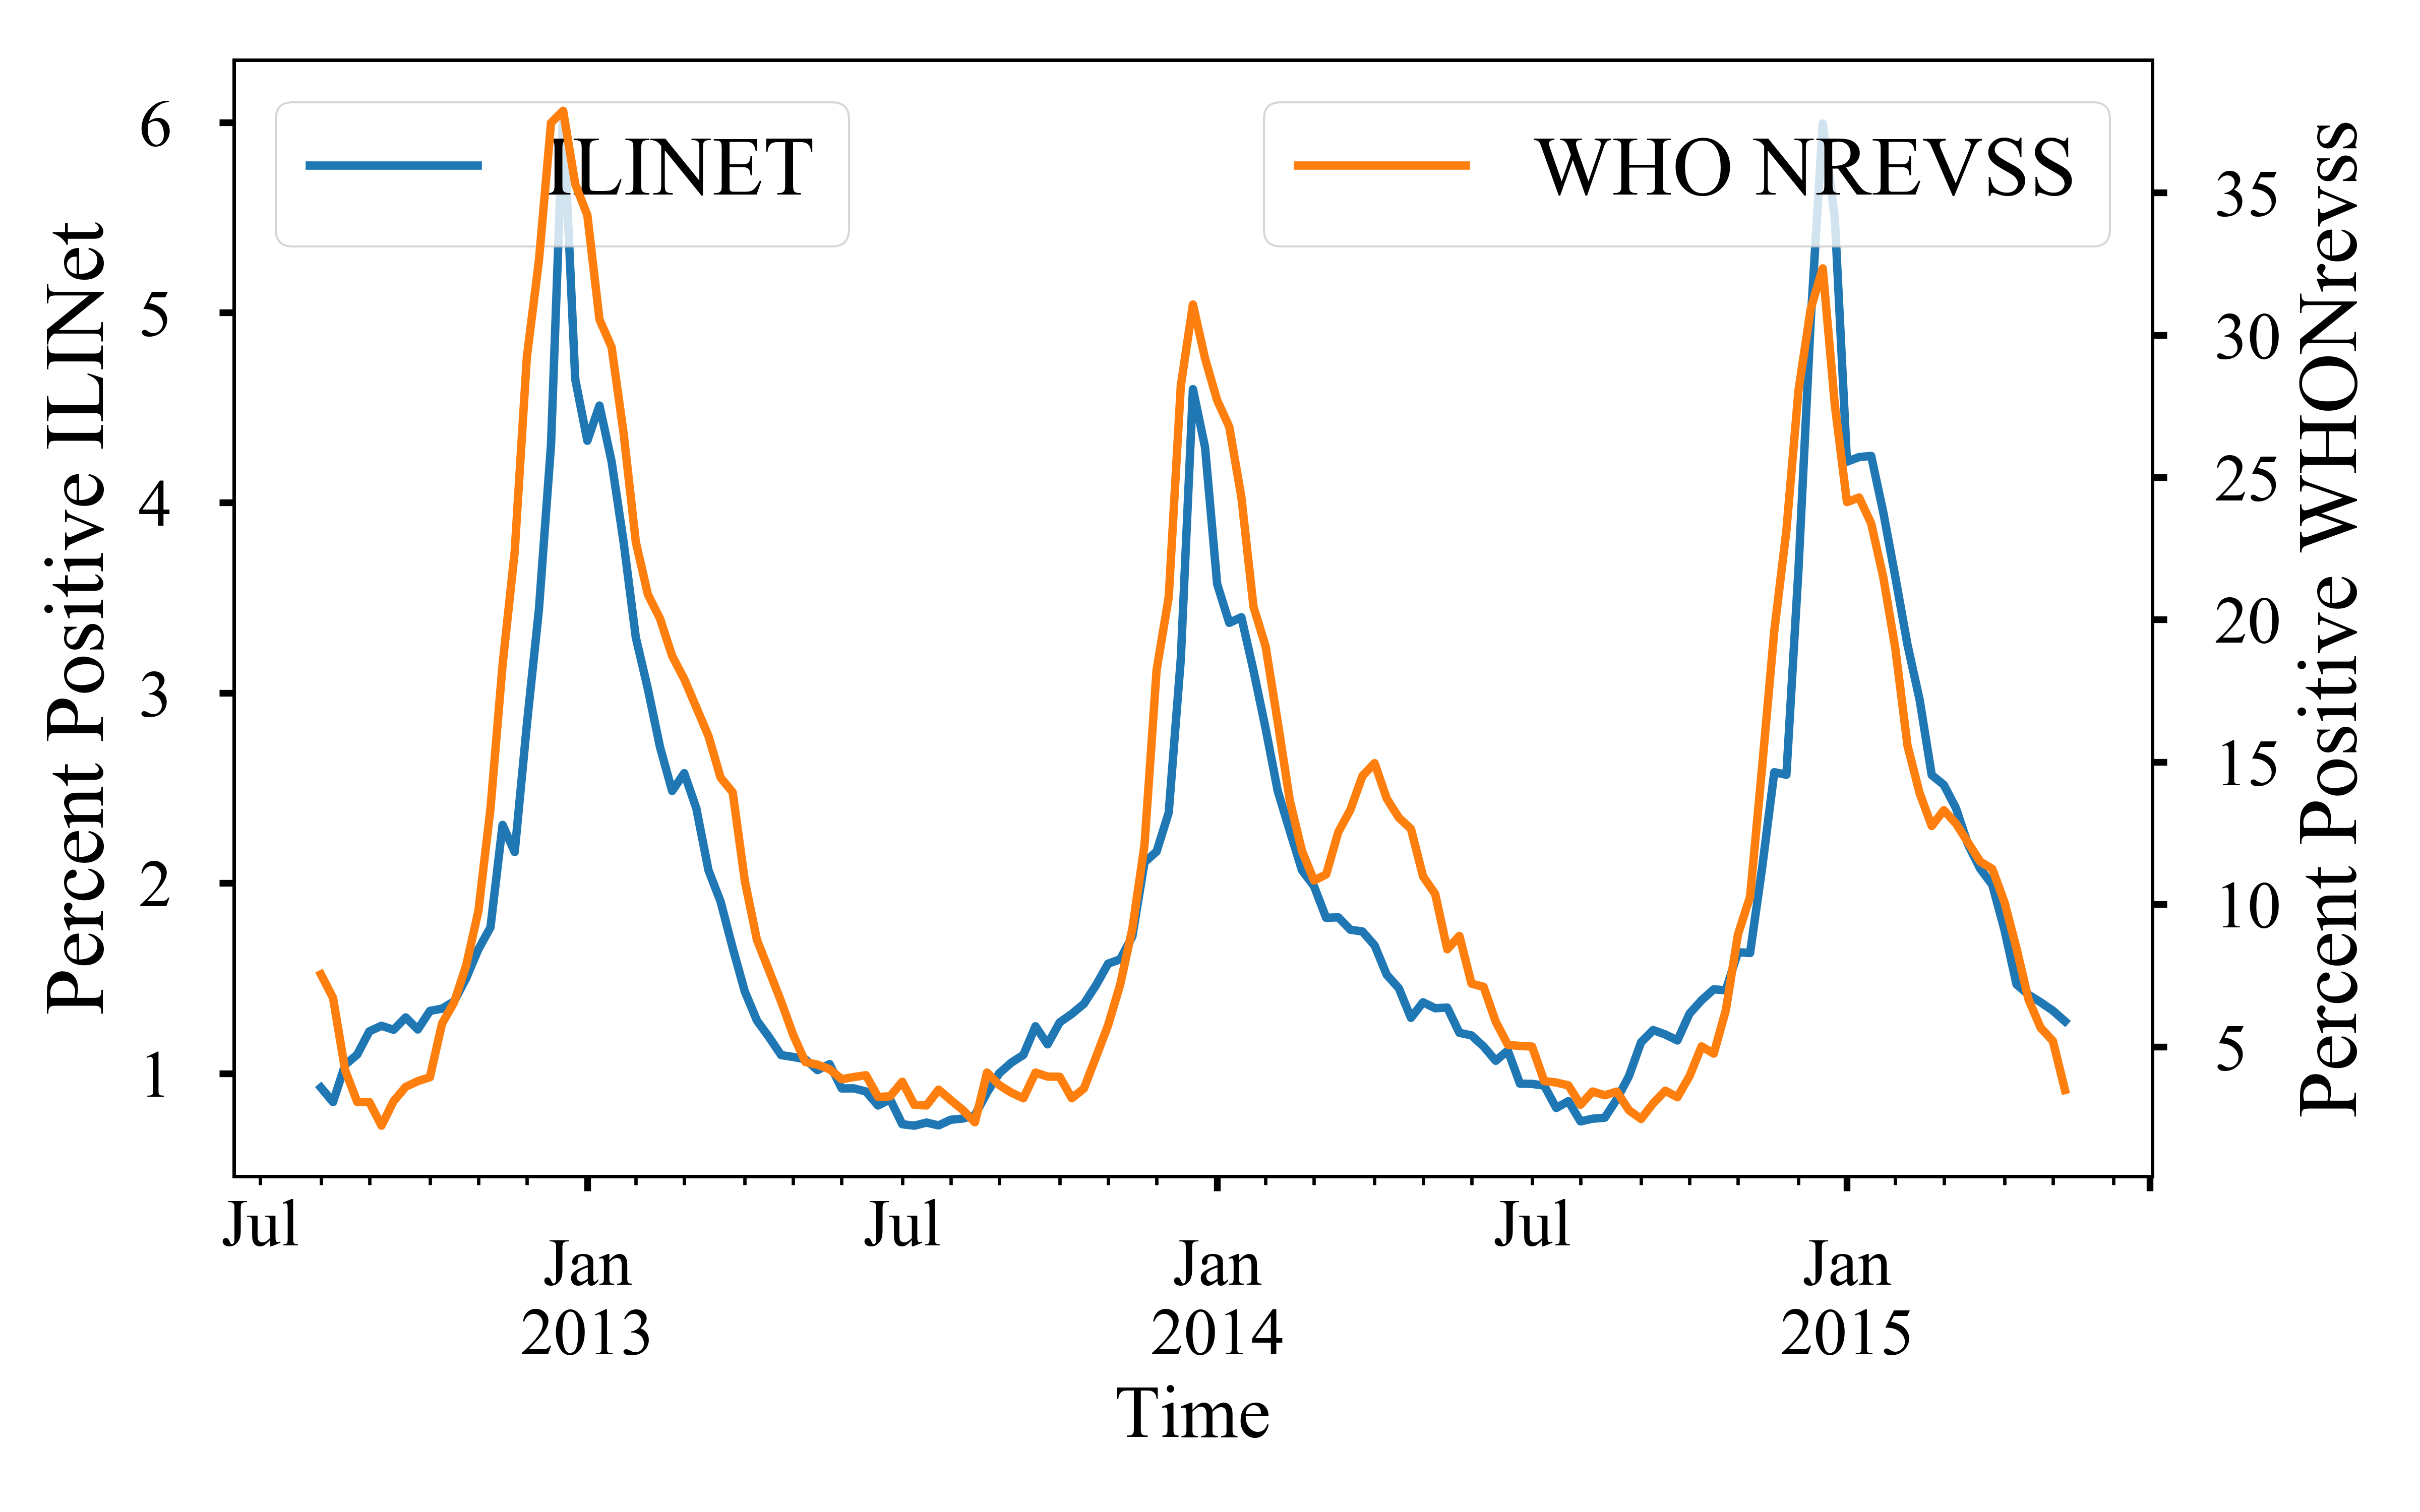
\includegraphics[width=0.9\textwidth]{./ilinet_vs_nrevss.png}
    \caption{Between surveillance difference}
    \end{center}
  \end{subfigure}
  \begin{subfigure}[t]{0.45\linewidth}
    \begin{center}
    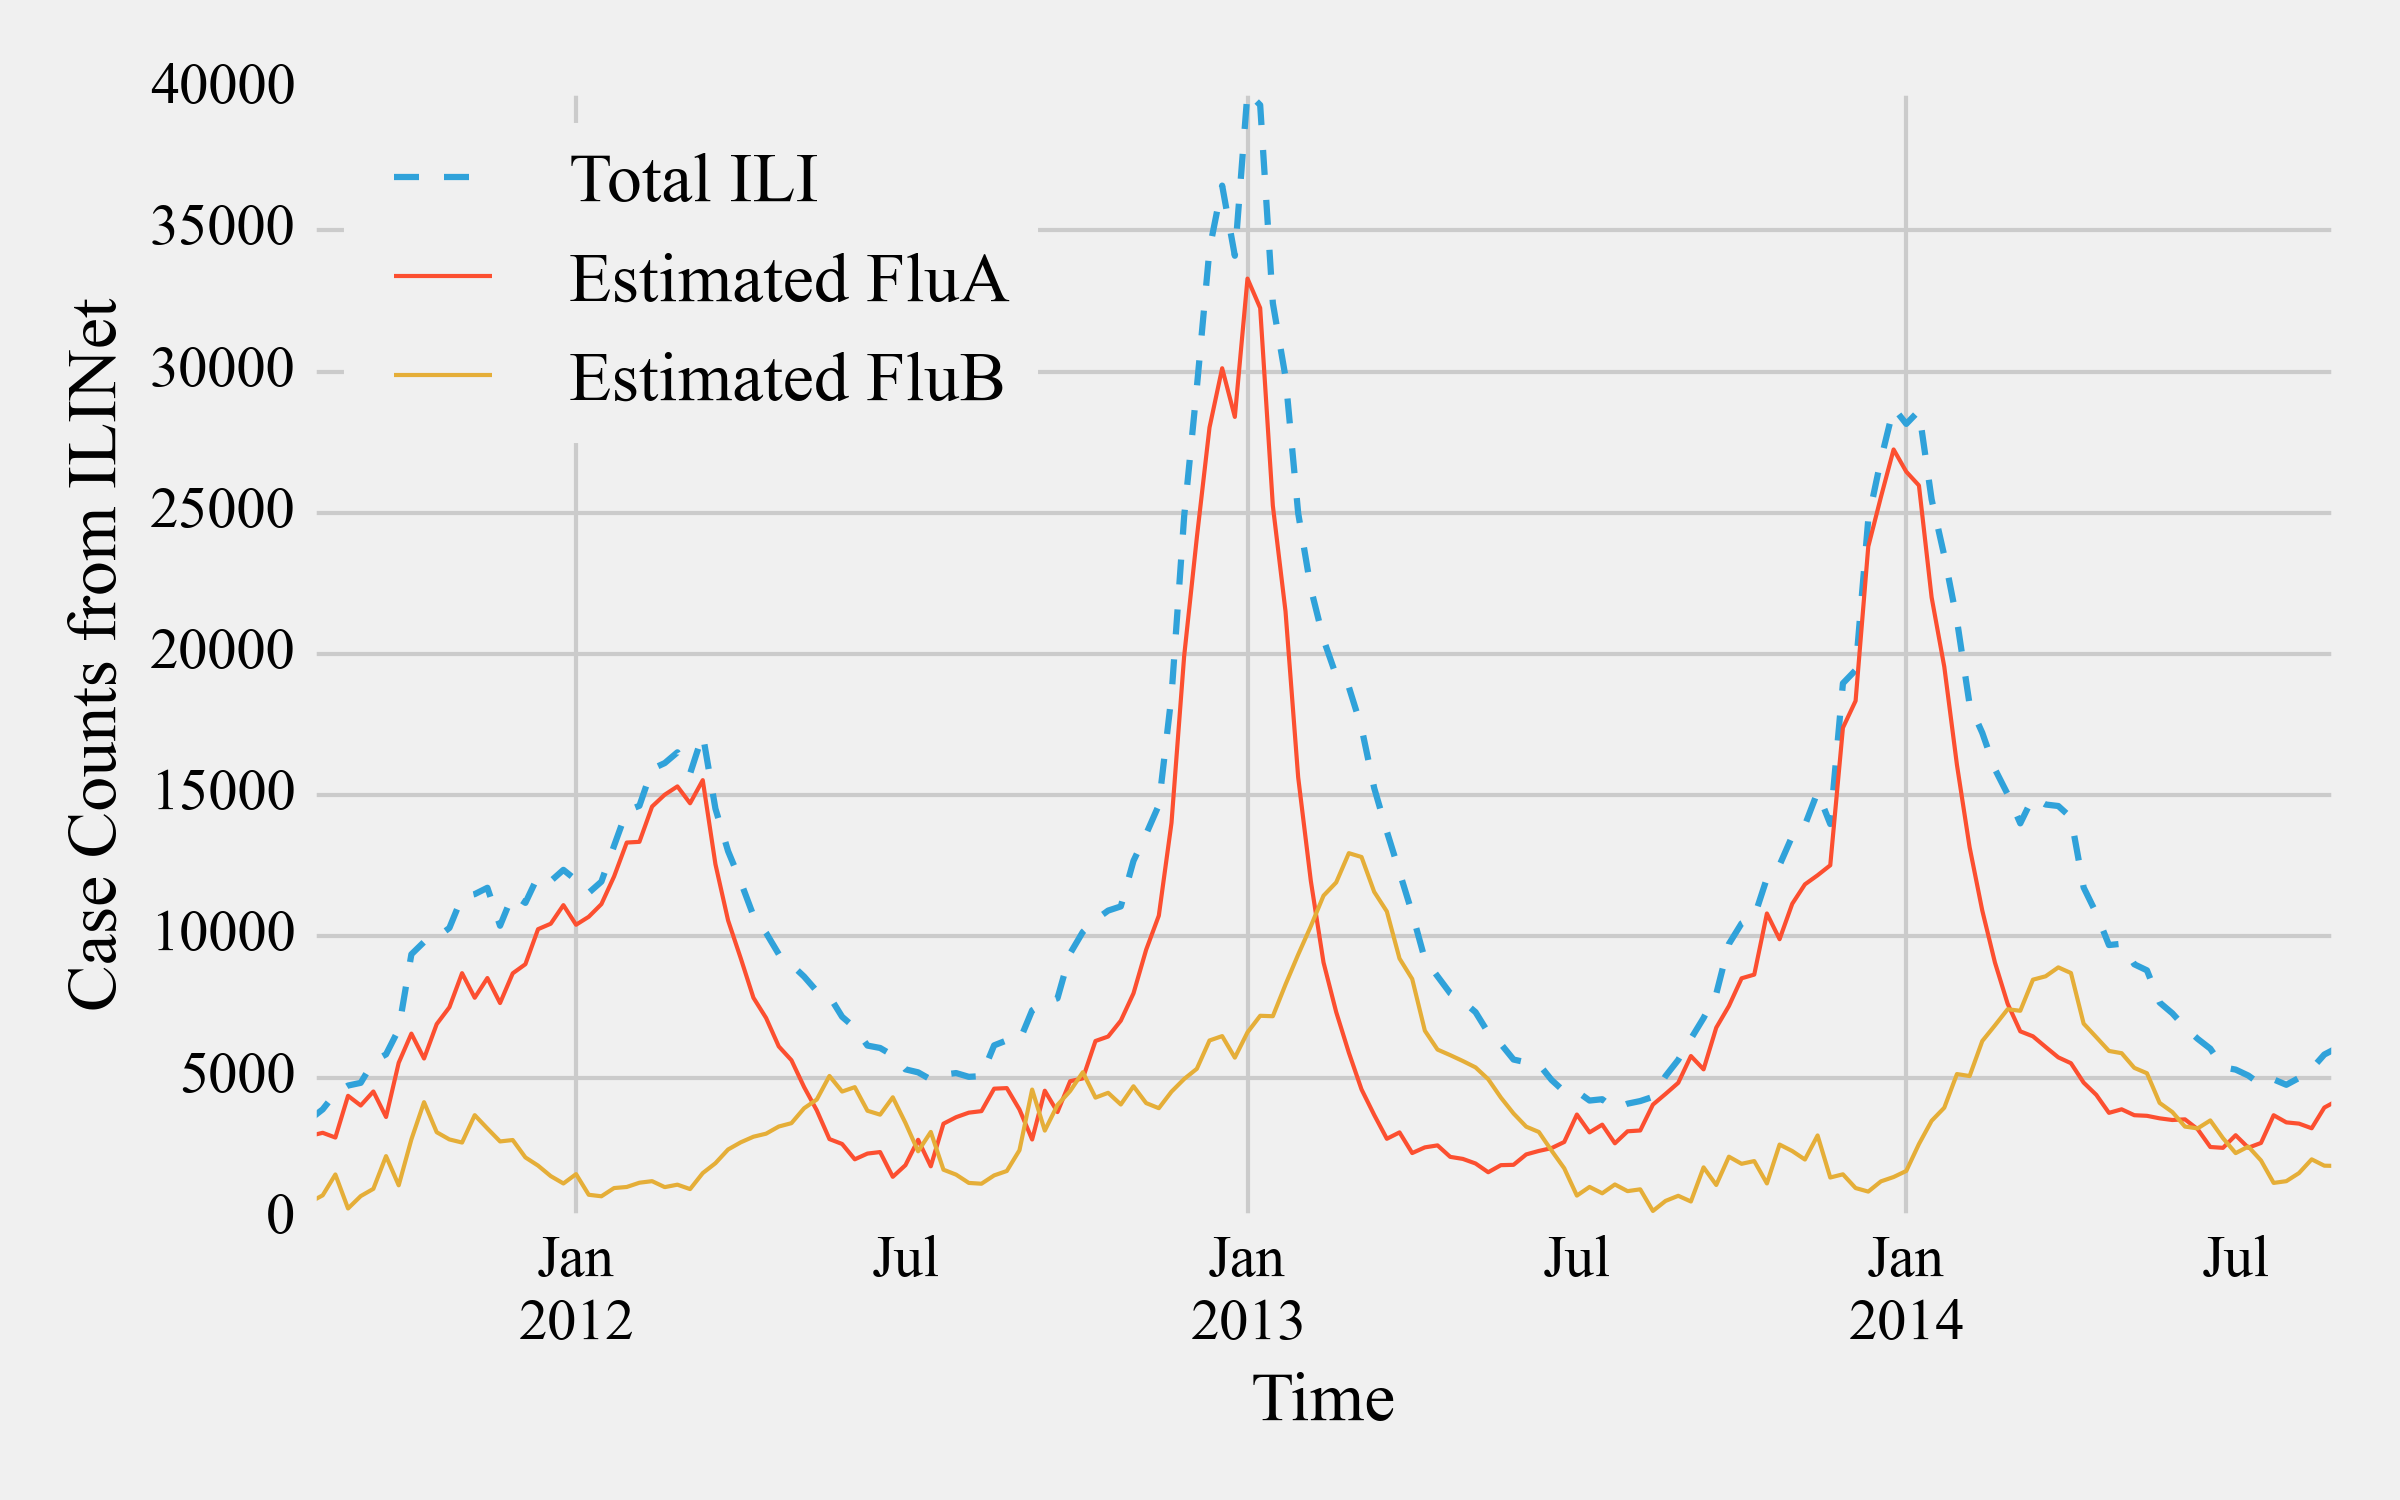
\includegraphics[width=0.9\textwidth]{./ilinet_subtyped.png}
    \caption{Between strains difference}
    \end{center}
  \end{subfigure}
  \\
  \begin{subfigure}[t]{0.45\linewidth}
    \begin{center}
    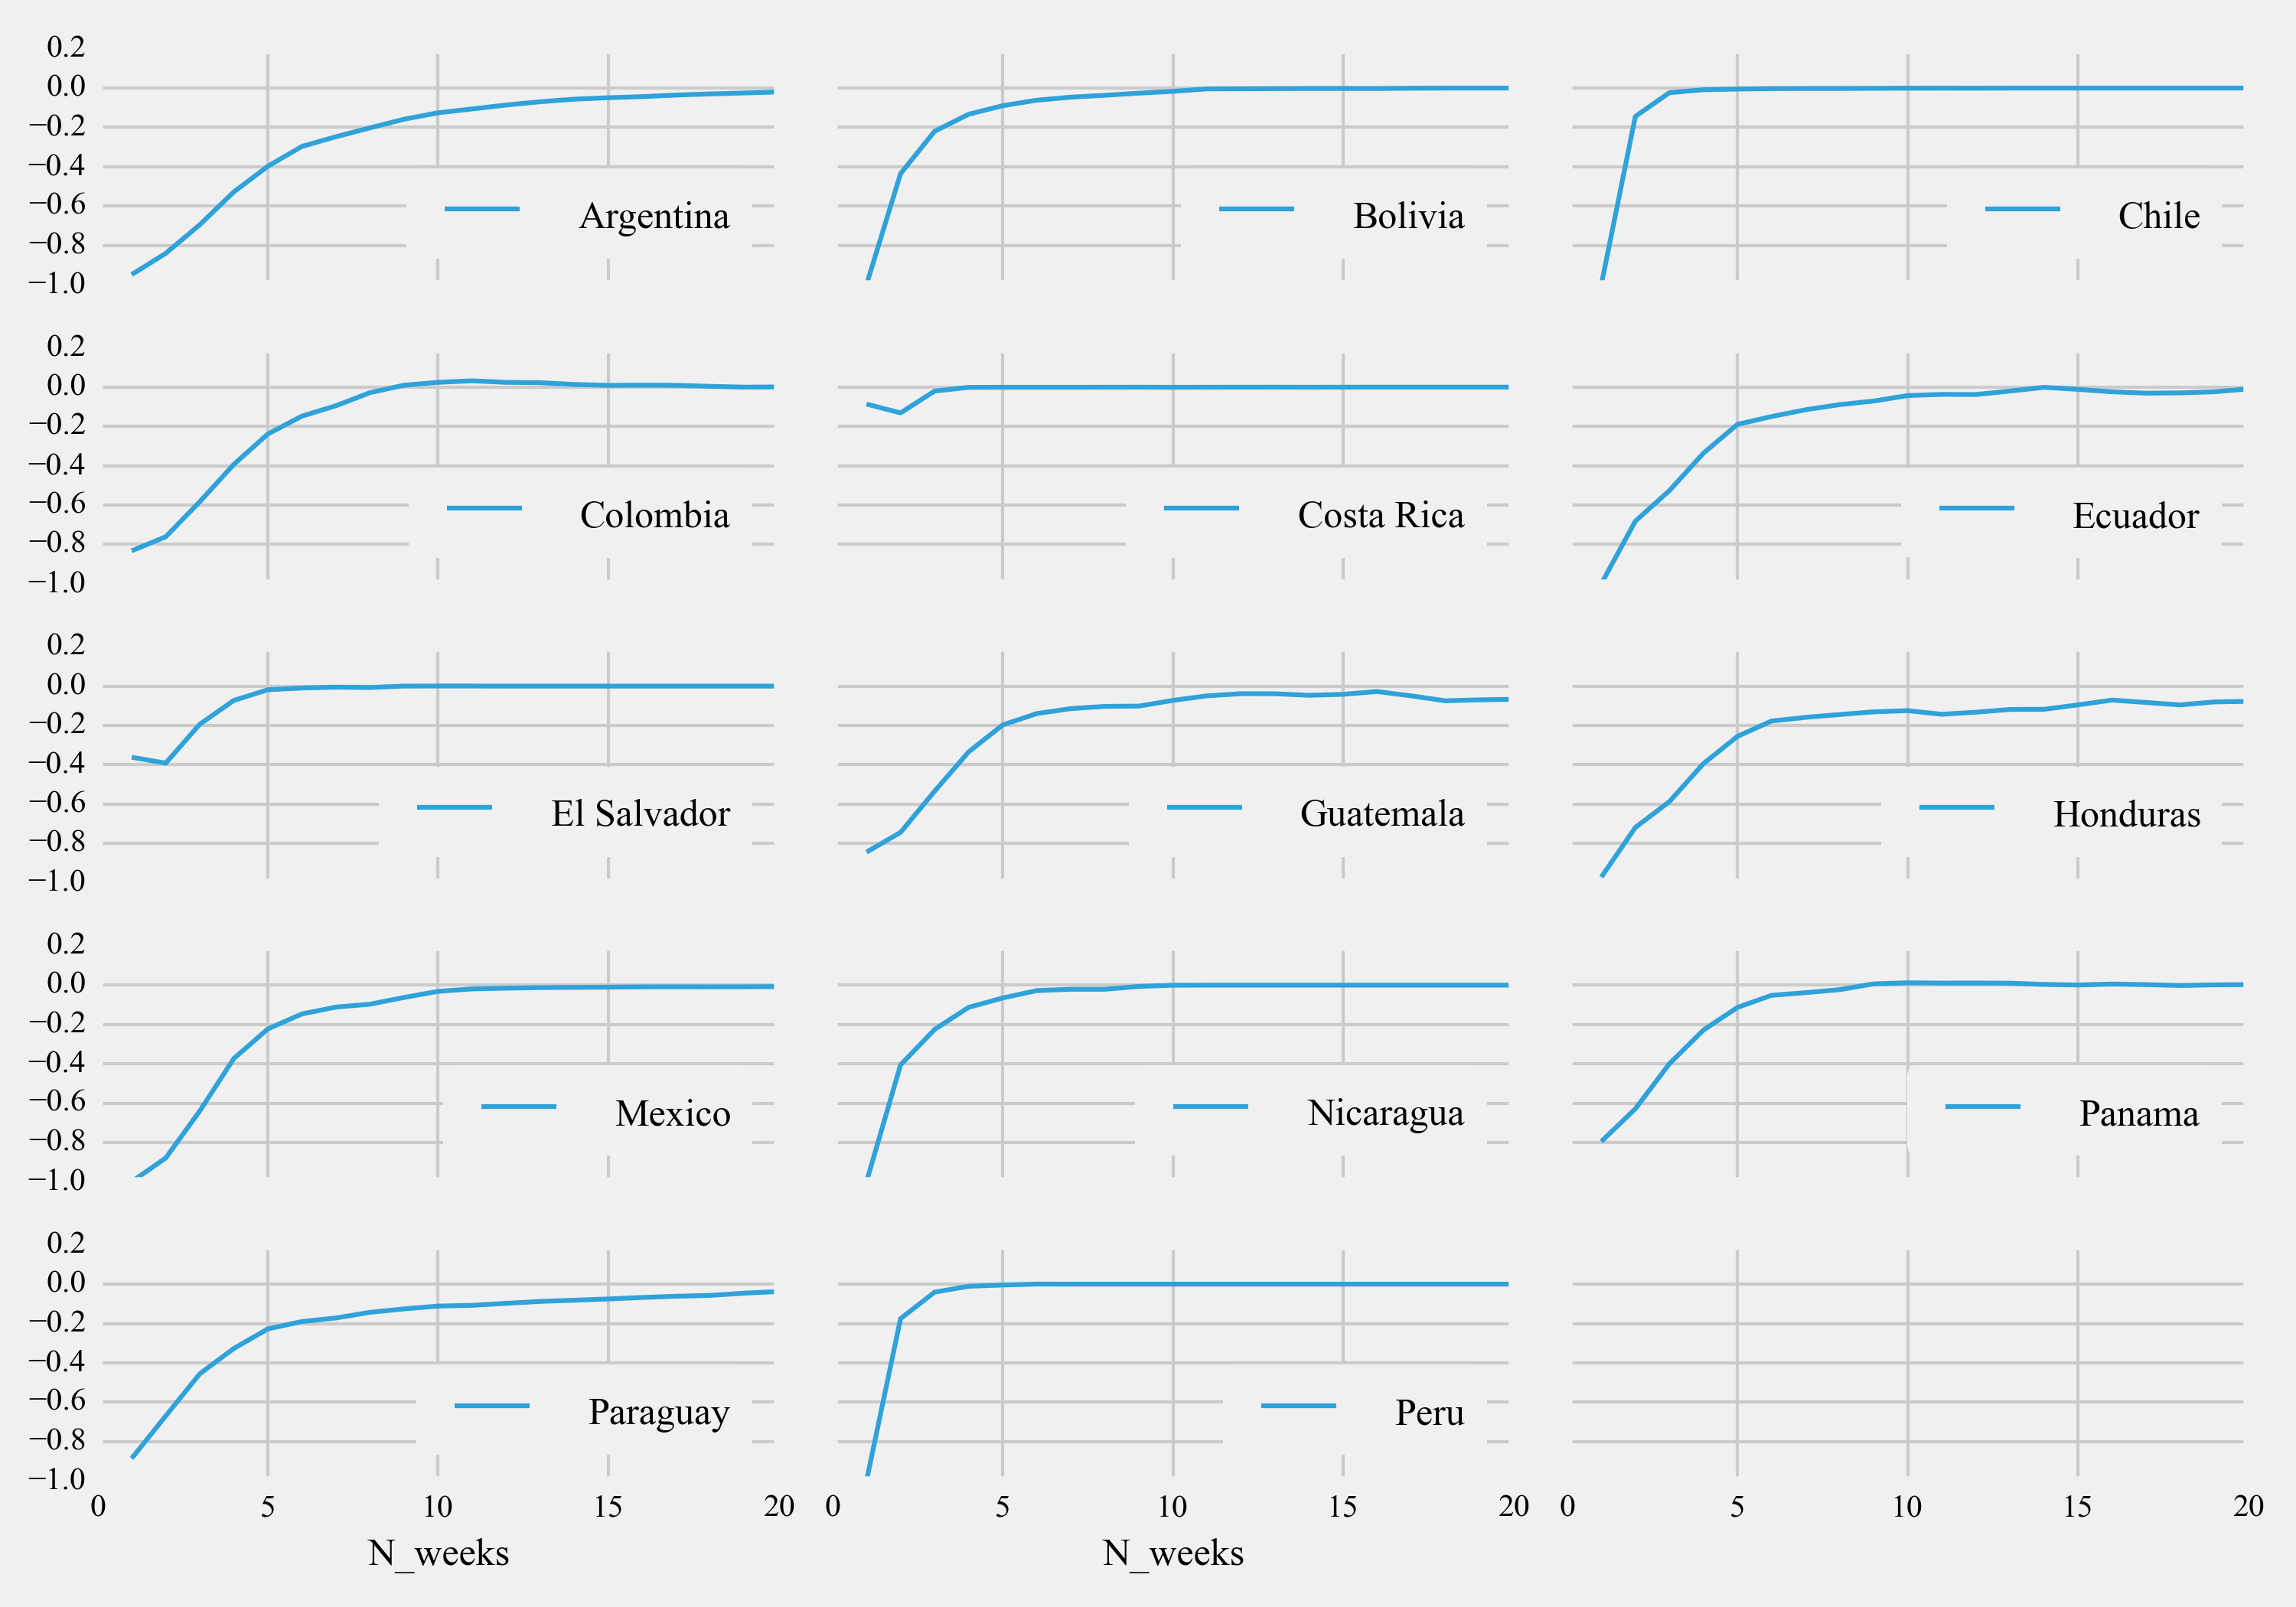
\includegraphics[width=0.9\textwidth]{./ili_updates.png}
    \caption{Surveillance Instability}
    \end{center}
  \end{subfigure}
  \begin{subfigure}[t]{0.45\linewidth}
    \begin{center}
    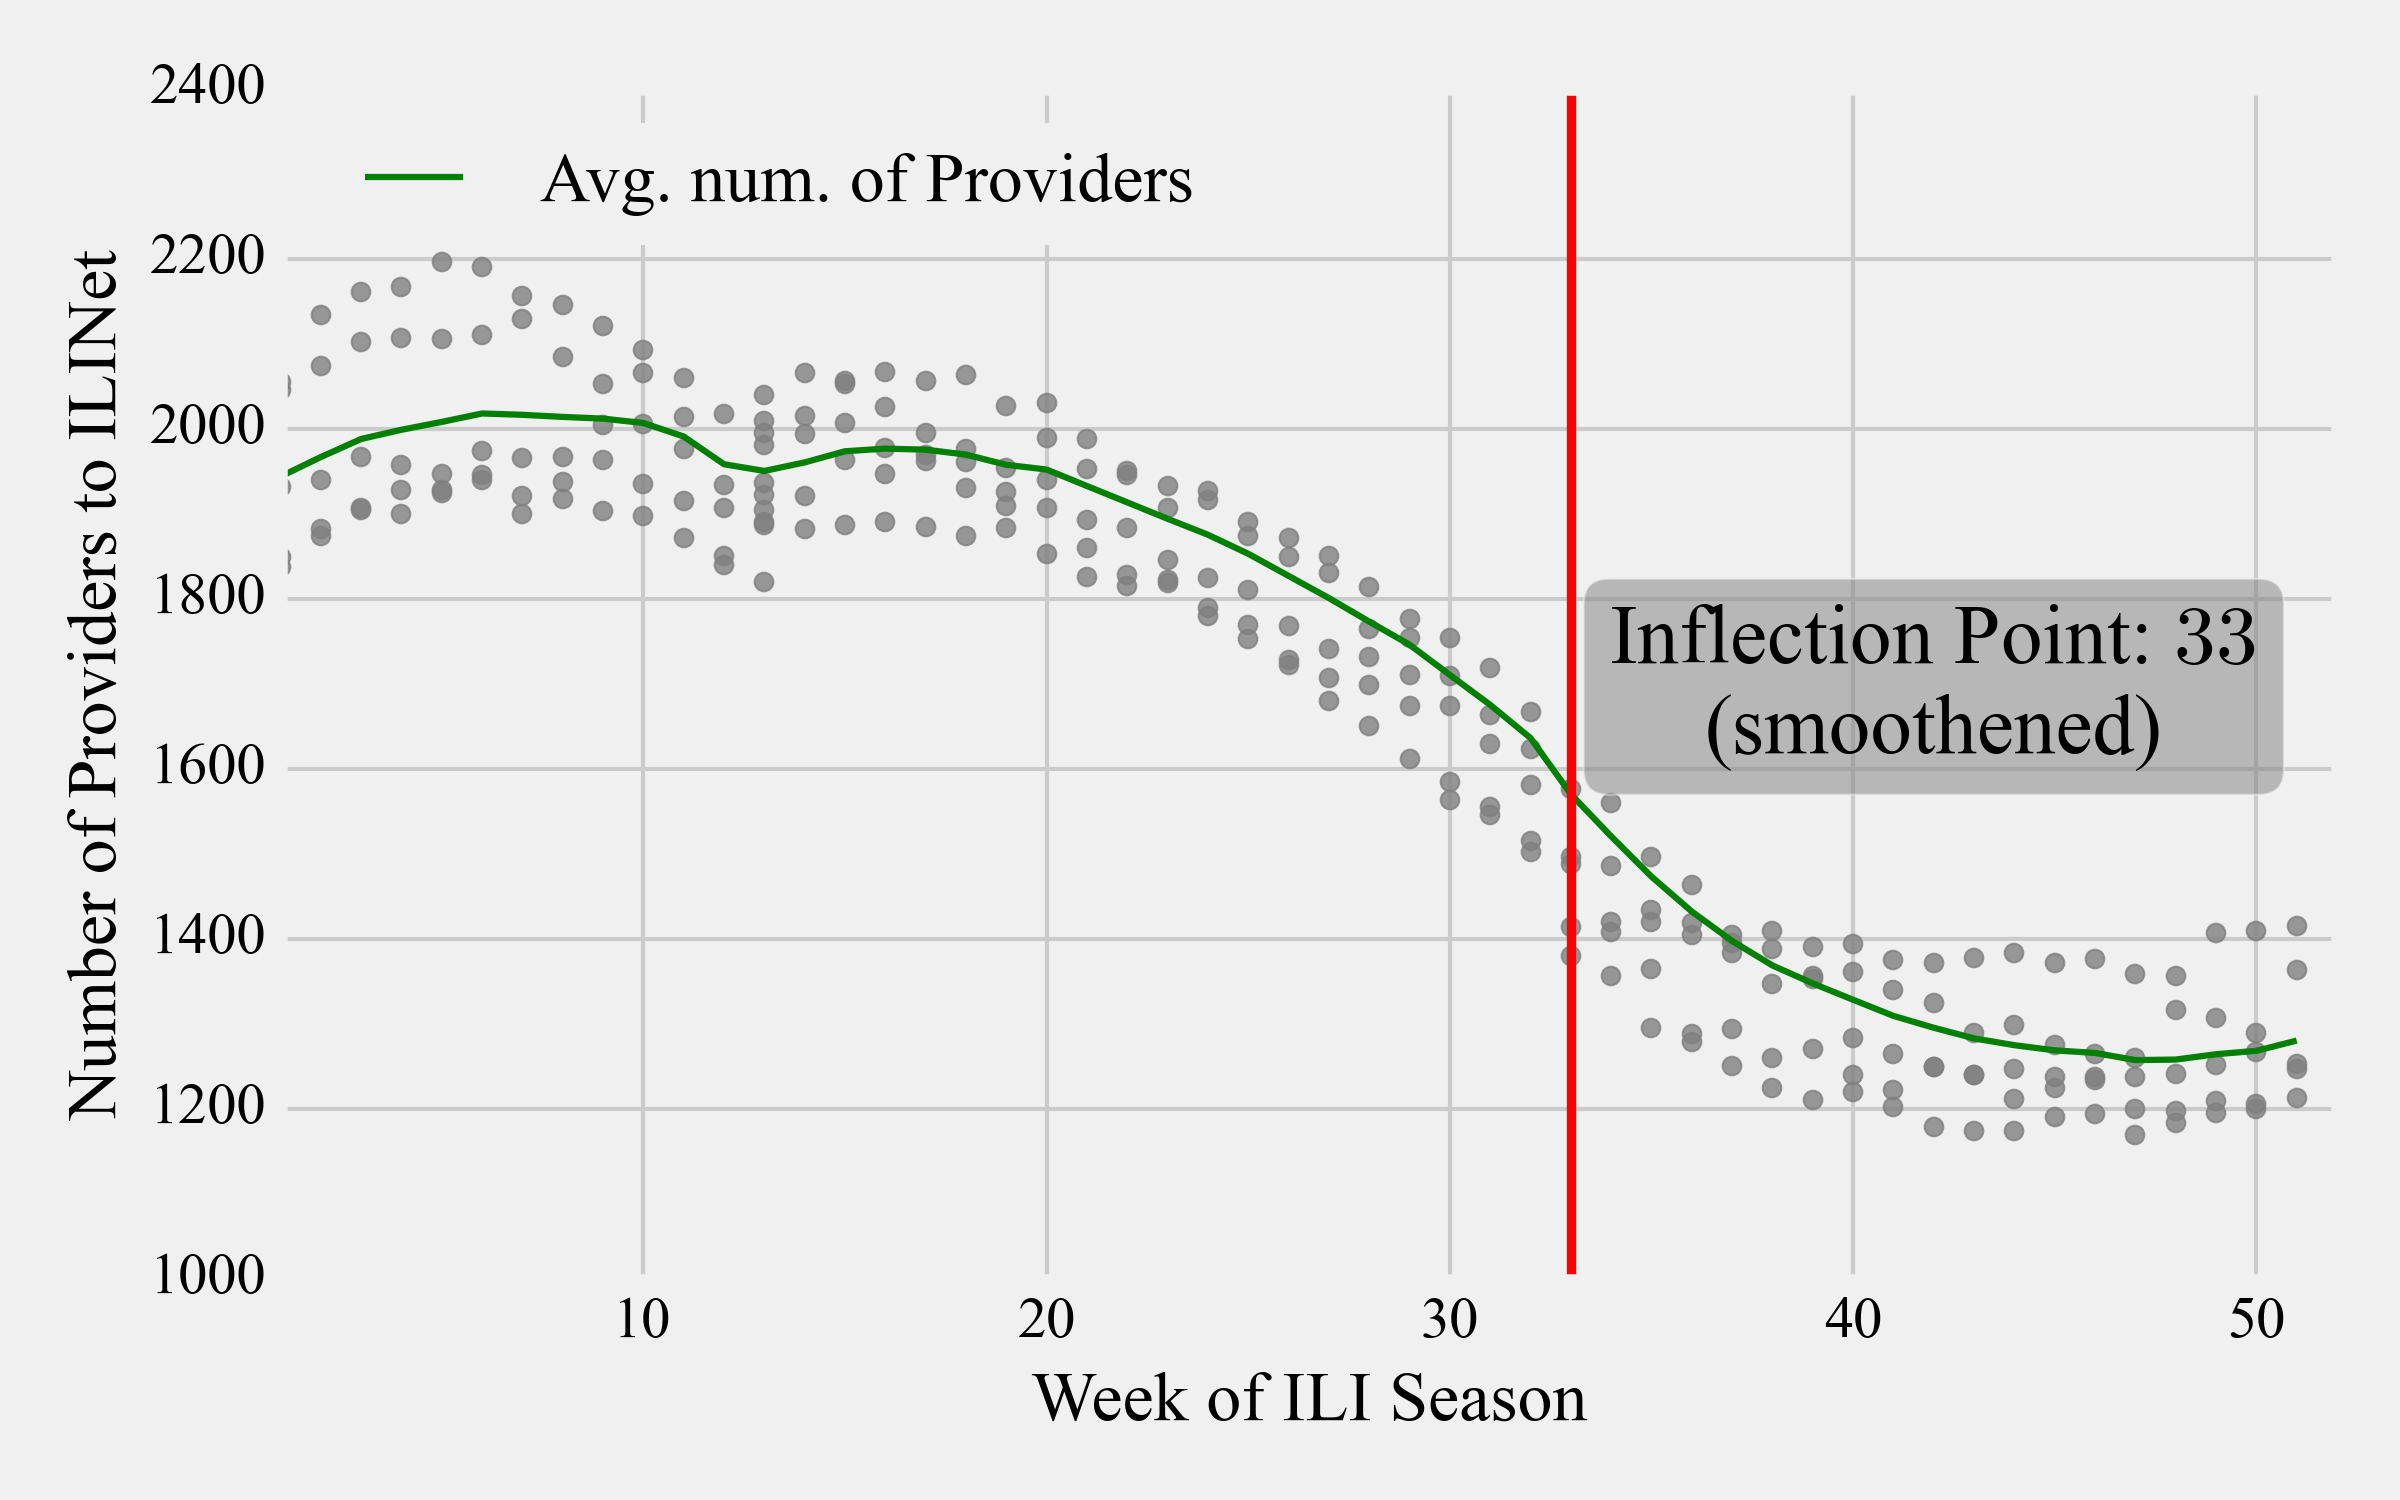
\includegraphics[width=0.9\textwidth]{./ili_surveillance_drop.png}
    \caption{Surveillance drop-off}
    \end{center}
  \end{subfigure}
  
\end{figure}


\end{document}
